\documentclass[tikz,border=10pt]{standalone}\usepackage{tikz}\usetikzlibrary{arrows.meta,positioning}\begin{document}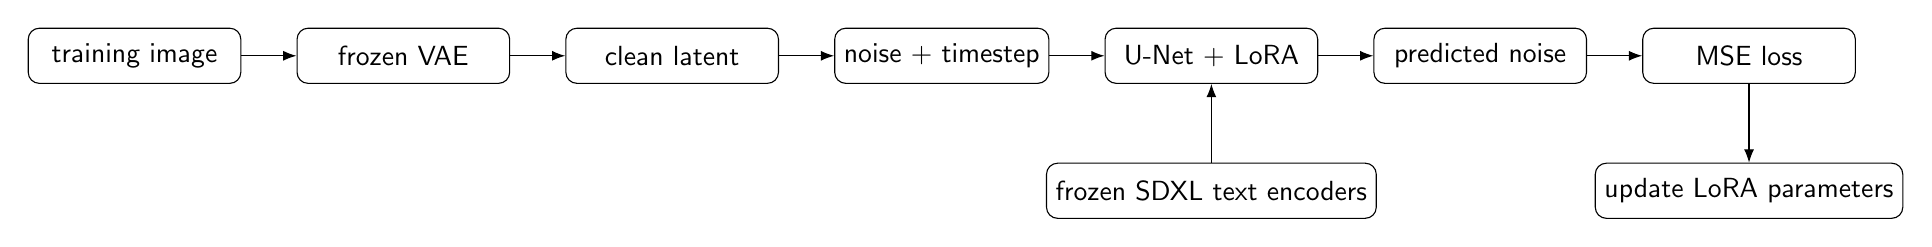
\begin{tikzpicture}[font=\sffamily,>=Latex,box/.style={draw,rounded corners,align=center,minimum width=2.7cm,minimum height=.7cm}]\node[box](im){training image};\node[box,right=.7cm of im](vae){frozen VAE};\node[box,right=.7cm of vae](lat){clean latent};\node[box,right=.7cm of lat](noise){noise + timestep};\node[box,right=.7cm of noise](unet){U-Net + LoRA};\node[box,right=.7cm of unet](pred){predicted noise};\node[box,right=.7cm of pred](loss){MSE loss};\draw[->](im)--(vae);\draw[->](vae)--(lat);\draw[->](lat)--(noise);\draw[->](noise)--(unet);\draw[->](unet)--(pred);\draw[->](pred)--(loss);\node[box,below=1cm of unet](text){frozen SDXL text encoders};\draw[->](text)--(unet);\node[box,below=1cm of loss](upd){update LoRA parameters};\draw[->](loss)--(upd);\end{tikzpicture}\end{document}
